\section{Pre-lab tasks}
% Q5.1
Using equation~\ref{math:Gammaf}, one finds
\begin{equation}
	\Gamma_e = \Gamma_\mu = \Gamma_\tau = \SI{83.40}{\mega\eV}
\end{equation}
The decay widths to leptons of three generations are the same because of lepton universality (neglecting mass). With the same equation, decay widths to quarks are
\begin{alignat*}{2}
	\Gamma_u &= \Gamma_c &&= \SI{285.34}{\mega\eV} \\
	\Gamma_d &= \Gamma_s = \Gamma_b &&= \SI{367.79}{\mega\eV}
\end{alignat*}
It is significantly larger, mainly because of more degrees of freedom (color) than leptons. Decays to neutrinos are invisible for detector in LEP, but still they have the width of
\begin{equation}
	\Gamma_{\nu} = \SI{165.84}{\mega\eV}
	\label{math:Gammanu}
\end{equation}

% Q5.2
Hadronic part in total
\begin{equation}
	\Gamma_\text{h} = \sum_{\forall q\neq t} \Gamma_q = \SI{1674.06}{\mega\eV}
\end{equation}
Charged decay
\begin{equation}
	\Gamma_\text{charged} = 3 \Gamma_e = \SI{250.17}{\mega\eV}
\end{equation}
Invisible decay
\begin{equation}
	\Gamma_\text{inv} = 3\Gamma_\nu = \SI{497.52}{\mega\eV}
\end{equation}
In total (except unknown decays)
\begin{equation}
	\Gamma_\text{total} = 3\Gamma_e + \Gamma_h + 3\Gamma_\nu = \SI{2421.75}{\mega\eV}
\end{equation}
These values are listed in table~\ref{tab:p_cross_theo}.
\begin{table}[ht]
	\centering
	\begin{tabular}{ccc}
		\toprule
		decay type & partial width[\si{\mega\eV}]  & partial cross section[$10^{-11}\si{\mega\eV\tothe{-2}}$] 	 \\
		\midrule
		hadronic & \num{1674.06} & \num{10.79} \\
		charged & \num{250.17} & \num{1.61} \\
		invisible & \num{497.52} & \num{3.21}  \\
		total & \num{2421.75} & \num{15.61} \\
		\bottomrule
	\end{tabular}
	\caption{Decays widths and partial cross sections\label{tab:p_cross_theo}}
\end{table}


% Q5.3
Assume that there is another generation of light fermions, the total width of $Z^0$ would be
\begin{equation}
	\Gamma'_\text{total} = \Gamma_\text{total} + \Gamma_e + \Gamma_\nu + \Gamma_u + \Gamma_d = \SI{3324.11}{\mega\eV}
\end{equation}
It would be a change of $37 \%$ percent!

% Q5.4
The differential cross section $\dv{\sigma}{\Omega}$ has different angular dependencies for $s$- and $t$-channels, see equations~\ref{math:diffCrossS} and~\ref{math:diffCrossT}. Simply plotting without the proportional constant in front shows where $s$- or $t$-channels dominates the process, see figure.~\ref{fig:angDep}.
\begin{figure}[ht]
	\centering
	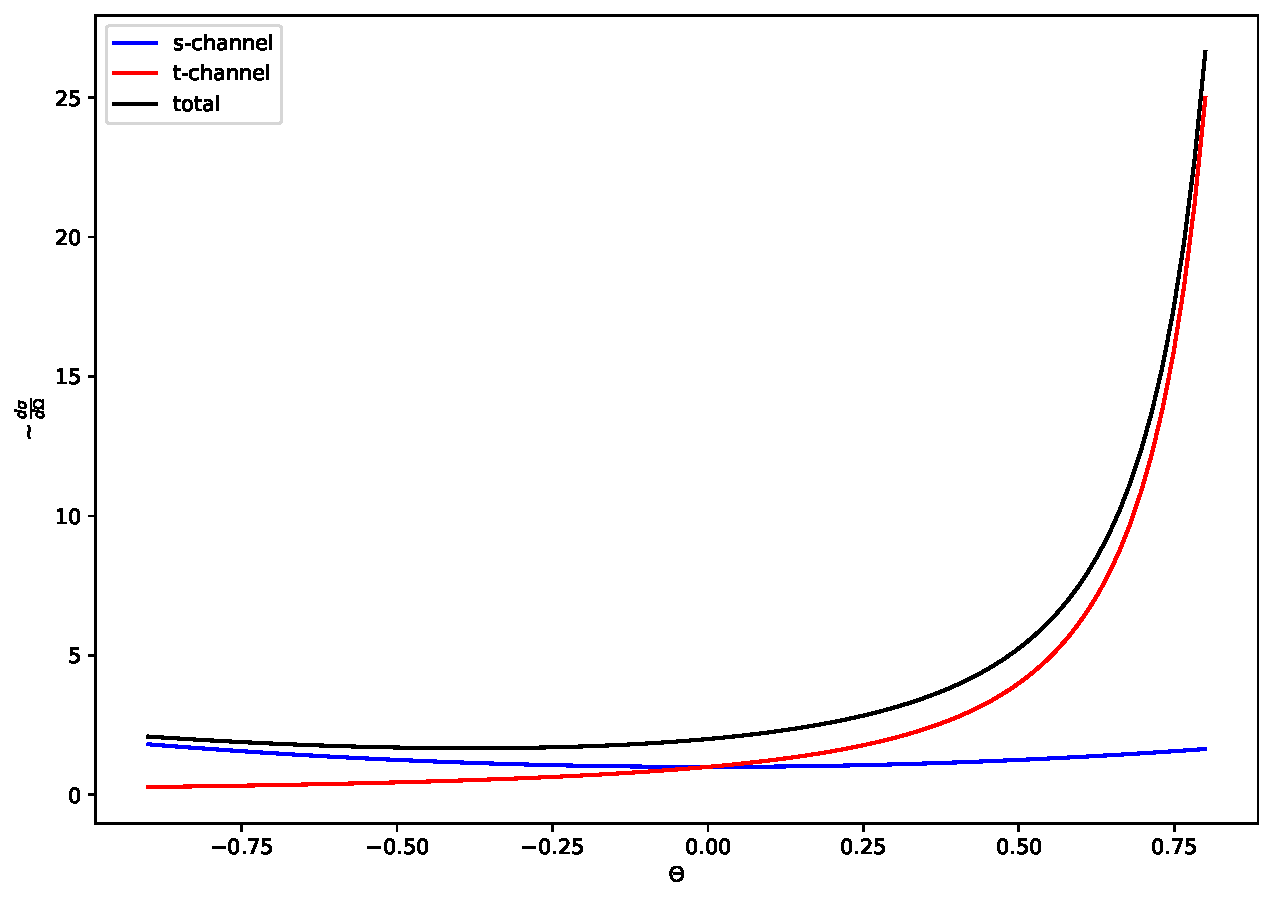
\includegraphics[width=0.8\linewidth]{angDep.pdf}
	\caption{Angular dependencies of two channels.}%
	\label{fig:angDep}
\end{figure}
At small angles, $t$-channel dominates, whereas at large angles, $s$-channel dominates.

%5.5
One can try to calculate the forward-backward asymmetry in $ Z^0 \rightarrow \mm$ channel with equation~\ref{math:AFBgen}. These are in table~\ref{tab:fbAsymm_theo}	
\begin{table}[htpb]
	\centering
\begin{tabular}{c|ccc}
	\toprule
	$\sqrt{s}$[\si{\giga\eV}] /$\sin^2(\theta_W)$ & \num{0.21} & \num{0.23} & \num{0.25} \\
	\midrule
	\num{89.225} & \num{-0.0379} & \num{-0.0420} & \num{-0.0451} \\
	\num{91.225} & \num{-0.0386} & \num{-0.0428} & \num{-0.0459} \\
	\num{93.225} & \num{-0.0394} & \num{-0.0436} & \num{-0.0468} \\
	\bottomrule
\end{tabular}
\caption{Forward-backward asymmetry in $Z^0\rightarrow \mm$ channel}
\label{tab:fbAsymm_theo}
\end{table}

